\documentclass{book}
\usepackage[a4paper,top=2.5cm,bottom=2.5cm,left=2.5cm,right=2.5cm]{geometry}
\usepackage{makeidx}
\usepackage{natbib}
\usepackage{graphicx}
\usepackage{multicol}
\usepackage{float}
\usepackage{listings}
\usepackage{color}
\usepackage{ifthen}
\usepackage[table]{xcolor}
\usepackage{textcomp}
\usepackage{alltt}
\usepackage{ifpdf}
\ifpdf
\usepackage[pdftex,
            pagebackref=true,
            colorlinks=true,
            linkcolor=blue,
            unicode
           ]{hyperref}
\else
\usepackage[ps2pdf,
            pagebackref=true,
            colorlinks=true,
            linkcolor=blue,
            unicode
           ]{hyperref}
\usepackage{pspicture}
\fi
\usepackage[utf8]{inputenc}
\usepackage{mathptmx}
\usepackage[scaled=.90]{helvet}
\usepackage{courier}
\usepackage{sectsty}
\usepackage{amssymb}
\usepackage[titles]{tocloft}
\usepackage{doxygen}
\lstset{language=C++,inputencoding=utf8,basicstyle=\footnotesize,breaklines=true,breakatwhitespace=true,tabsize=4,numbers=left }
\makeindex
\setcounter{tocdepth}{3}
\renewcommand{\footrulewidth}{0.4pt}
\renewcommand{\familydefault}{\sfdefault}
\hfuzz=15pt
\setlength{\emergencystretch}{15pt}
\hbadness=750
\tolerance=750
\begin{document}
\hypersetup{pageanchor=false,citecolor=blue}
\begin{titlepage}
\vspace*{7cm}
\begin{center}
{\Large My Project }\\
\vspace*{1cm}
{\large Generated by Doxygen 1.8.2}\\
\vspace*{0.5cm}
{\small Tue Nov 27 2012 14:03:21}\\
\end{center}
\end{titlepage}
\clearemptydoublepage
\pagenumbering{roman}
\tableofcontents
\clearemptydoublepage
\pagenumbering{arabic}
\hypersetup{pageanchor=true,citecolor=blue}
\chapter{Hierarchical Index}
\section{Class Hierarchy}
This inheritance list is sorted roughly, but not completely, alphabetically\-:\begin{DoxyCompactList}
\item \contentsline{section}{Best\-First\-Search\-Node}{\pageref{class_best_first_search_node}}{}
\item \contentsline{section}{Point2d}{\pageref{struct_point2d}}{}
\item \contentsline{section}{Point2\-D}{\pageref{class_point2_d}}{}
\item Q\-Graphics\-Ellipse\-Item\begin{DoxyCompactList}
\item \contentsline{section}{Agent}{\pageref{class_agent}}{}
\item \contentsline{section}{Goal\-Point}{\pageref{class_goal_point}}{}
\end{DoxyCompactList}
\item Q\-Graphics\-Polygon\-Item\begin{DoxyCompactList}
\item \contentsline{section}{Obstacle}{\pageref{class_obstacle}}{}
\end{DoxyCompactList}
\item Q\-Graphics\-Rect\-Item\begin{DoxyCompactList}
\item \contentsline{section}{Potential\-Field}{\pageref{class_potential_field}}{}
\end{DoxyCompactList}
\item Q\-Main\-Window\begin{DoxyCompactList}
\item \contentsline{section}{Main\-Window}{\pageref{class_main_window}}{}
\end{DoxyCompactList}
\item Q\-Thread\begin{DoxyCompactList}
\item \contentsline{section}{Potential\-Field\-Worker}{\pageref{class_potential_field_worker}}{}
\end{DoxyCompactList}
\item Q\-Widget\begin{DoxyCompactList}
\item \contentsline{section}{Playground}{\pageref{class_playground}}{}
\end{DoxyCompactList}
\item \contentsline{section}{Triangle}{\pageref{struct_triangle}}{}
\end{DoxyCompactList}

\chapter{Class Index}
\section{Class List}
Here are the classes, structs, unions and interfaces with brief descriptions\-:\begin{DoxyCompactList}
\item\contentsline{section}{\hyperlink{class_agent}{Agent} \\*Class that holds info about an agent }{\pageref{class_agent}}{}
\item\contentsline{section}{\hyperlink{class_best_first_search_node}{Best\-First\-Search\-Node} }{\pageref{class_best_first_search_node}}{}
\item\contentsline{section}{\hyperlink{class_goal_point}{Goal\-Point} }{\pageref{class_goal_point}}{}
\item\contentsline{section}{\hyperlink{class_main_window}{Main\-Window} }{\pageref{class_main_window}}{}
\item\contentsline{section}{\hyperlink{class_obstacle}{Obstacle} }{\pageref{class_obstacle}}{}
\item\contentsline{section}{\hyperlink{class_playground}{Playground} }{\pageref{class_playground}}{}
\item\contentsline{section}{\hyperlink{struct_point2d}{Point2d} }{\pageref{struct_point2d}}{}
\item\contentsline{section}{\hyperlink{class_point2_d}{Point2\-D} }{\pageref{class_point2_d}}{}
\item\contentsline{section}{\hyperlink{class_potential_field}{Potential\-Field} }{\pageref{class_potential_field}}{}
\item\contentsline{section}{\hyperlink{class_potential_field_worker}{Potential\-Field\-Worker} }{\pageref{class_potential_field_worker}}{}
\item\contentsline{section}{\hyperlink{struct_triangle}{Triangle} }{\pageref{struct_triangle}}{}
\end{DoxyCompactList}

\chapter{File Index}
\section{File List}
Here is a list of all documented files with brief descriptions\-:\begin{DoxyCompactList}
\item\contentsline{section}{\hyperlink{_agent_8h}{Agent.\-h} \\*Contains \hyperlink{class_agent}{Agent} class }{\pageref{_agent_8h}}{}
\item\contentsline{section}{\hyperlink{_best_first_search_node_8h}{Best\-First\-Search\-Node.\-h} \\*Contains \hyperlink{class_best_first_search_node}{Best\-First\-Search\-Node} class }{\pageref{_best_first_search_node_8h}}{}
\item\contentsline{section}{\hyperlink{_goal_point_8h}{Goal\-Point.\-h} \\*Contains \hyperlink{class_goal_point}{Goal\-Point} class declaration }{\pageref{_goal_point_8h}}{}
\item\contentsline{section}{\hyperlink{gpu_potential_fields_wrapper_8h}{gpu\-Potential\-Fields\-Wrapper.\-h} \\*Contains functions which uses G\-P\-U }{\pageref{gpu_potential_fields_wrapper_8h}}{}
\item\contentsline{section}{\hyperlink{_main_window_8h}{Main\-Window.\-h} \\*Contains \hyperlink{class_main_window}{Main\-Window} class }{\pageref{_main_window_8h}}{}
\item\contentsline{section}{\hyperlink{_obstacle_8h}{Obstacle.\-h} \\*Contains \hyperlink{class_obstacle}{Obstacle} class }{\pageref{_obstacle_8h}}{}
\item\contentsline{section}{\hyperlink{_playground_8h}{Playground.\-h} \\*Contains \hyperlink{class_playground}{Playground} class }{\pageref{_playground_8h}}{}
\item\contentsline{section}{\hyperlink{_point2_d_8h}{Point2\-D.\-h} \\*Simple \hyperlink{class_point2_d}{Point2\-D} class }{\pageref{_point2_d_8h}}{}
\item\contentsline{section}{\hyperlink{_potential_field_8h}{Potential\-Field.\-h} \\*Contains \hyperlink{class_potential_field}{Potential\-Field} class }{\pageref{_potential_field_8h}}{}
\item\contentsline{section}{\hyperlink{_potential_field_worker_8h}{Potential\-Field\-Worker.\-h} \\*Contains \hyperlink{class_potential_field_worker}{Potential\-Field\-Worker} class for thread }{\pageref{_potential_field_worker_8h}}{}
\item\contentsline{section}{\hyperlink{_triangle_8h}{Triangle.\-h} \\*Contains \hyperlink{struct_triangle}{Triangle} class and few global constants }{\pageref{_triangle_8h}}{}
\end{DoxyCompactList}

\chapter{Class Documentation}
\hypertarget{class_agent}{\section{Agent Class Reference}
\label{class_agent}\index{Agent@{Agent}}
}


Class that holds info about an agent.  




{\ttfamily \#include $<$Agent.\-h$>$}

Inheritance diagram for Agent\-:\begin{figure}[H]
\begin{center}
\leavevmode
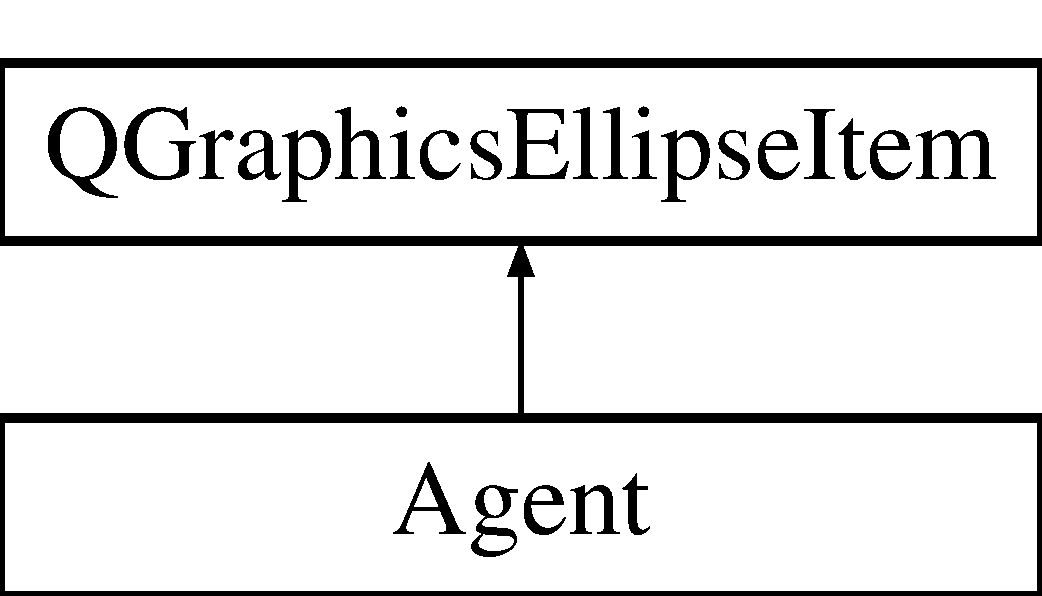
\includegraphics[height=2.000000cm]{class_agent}
\end{center}
\end{figure}
\subsection*{Public Member Functions}
\begin{DoxyCompactItemize}
\item 
\hyperlink{class_agent_ae94d885a5f3900b0b67927710945ba26}{Agent} (qreal x, qreal y, qreal width, qreal height, Q\-Graphics\-Item $\ast$parent=0)
\begin{DoxyCompactList}\small\item\em Constructor. \end{DoxyCompactList}\item 
\hypertarget{class_agent_affa8c88292795f1f07e7ac74ef50cb6f}{virtual void {\bfseries paint} (Q\-Painter $\ast$painter, const Q\-Style\-Option\-Graphics\-Item $\ast$option, Q\-Widget $\ast$widget=0)}\label{class_agent_affa8c88292795f1f07e7ac74ef50cb6f}

\item 
void \hyperlink{class_agent_a6a9ff6b09b8a66177a90f0172c72a884}{Tick} (int millis)
\begin{DoxyCompactList}\small\item\em Tick. \end{DoxyCompactList}\item 
\hypertarget{class_agent_af388a0b175ceda73e1834e399f6f98e9}{void {\bfseries Set\-Goal} (int \-\_\-goal\-X, int \-\_\-goal\-Y)}\label{class_agent_af388a0b175ceda73e1834e399f6f98e9}

\item 
\hypertarget{class_agent_a3037f3d0b54aaf8272c176c26d096c26}{int {\bfseries Goal\-X} ()}\label{class_agent_a3037f3d0b54aaf8272c176c26d096c26}

\item 
\hypertarget{class_agent_a0a87900958ea46f2e15df2c9f42e976e}{int {\bfseries Goal\-Y} ()}\label{class_agent_a0a87900958ea46f2e15df2c9f42e976e}

\item 
\hypertarget{class_agent_acfbcafe677bc8810fac4f8311e0d9c3f}{\hyperlink{class_point2_d}{Point2\-D} {\bfseries Real\-Pos} ()}\label{class_agent_acfbcafe677bc8810fac4f8311e0d9c3f}

\item 
\hypertarget{class_agent_ad886fc8c1e03592b23296cd82d8b0dbb}{\hyperlink{class_point2_d}{Point2\-D} {\bfseries Field\-Center} ()}\label{class_agent_ad886fc8c1e03592b23296cd82d8b0dbb}

\item 
\hypertarget{class_agent_a610a51c9fd807c1d75107409f1a6a8e0}{void {\bfseries Set\-Path} (stack$<$ \hyperlink{class_point2_d}{Point2\-D} $>$ $\ast$\-\_\-path)}\label{class_agent_a610a51c9fd807c1d75107409f1a6a8e0}

\end{DoxyCompactItemize}


\subsection{Detailed Description}
Class that holds info about an agent. 

This class contains information about the agen, i.\-e. its position, velocity, goal, current path. 

\subsection{Constructor \& Destructor Documentation}
\hypertarget{class_agent_ae94d885a5f3900b0b67927710945ba26}{\index{Agent@{Agent}!Agent@{Agent}}
\index{Agent@{Agent}!Agent@{Agent}}
\subsubsection[{Agent}]{\setlength{\rightskip}{0pt plus 5cm}Agent\-::\-Agent (
\begin{DoxyParamCaption}
\item[{qreal}]{x, }
\item[{qreal}]{y, }
\item[{qreal}]{width, }
\item[{qreal}]{height, }
\item[{Q\-Graphics\-Item $\ast$}]{parent = {\ttfamily 0}}
\end{DoxyParamCaption}
)}}\label{class_agent_ae94d885a5f3900b0b67927710945ba26}


Constructor. 

Creates a new agent with given position, width and height of ellipse.


\begin{DoxyParams}[1]{Parameters}
\mbox{\tt in}  & {\em x} & Origin x position \\
\hline
\mbox{\tt in}  & {\em y} & Origin y position \\
\hline
\mbox{\tt in}  & {\em width} & \hyperlink{class_agent}{Agent} width \\
\hline
\mbox{\tt in}  & {\em height} & \hyperlink{class_agent}{Agent} height \\
\hline
\mbox{\tt in}  & {\em parent} & possible Q\-Graphics\-Item parent \\
\hline
\end{DoxyParams}


\subsection{Member Function Documentation}
\hypertarget{class_agent_a6a9ff6b09b8a66177a90f0172c72a884}{\index{Agent@{Agent}!Tick@{Tick}}
\index{Tick@{Tick}!Agent@{Agent}}
\subsubsection[{Tick}]{\setlength{\rightskip}{0pt plus 5cm}void Agent\-::\-Tick (
\begin{DoxyParamCaption}
\item[{int}]{millis}
\end{DoxyParamCaption}
)}}\label{class_agent_a6a9ff6b09b8a66177a90f0172c72a884}


Tick. 

Updates agent position towards goal.


\begin{DoxyParams}[1]{Parameters}
\mbox{\tt in}  & {\em millis} & How many milliseconds lasted from last tick. \\
\hline
\end{DoxyParams}


The documentation for this class was generated from the following files\-:\begin{DoxyCompactItemize}
\item 
\hyperlink{_agent_8h}{Agent.\-h}\item 
Agent.\-cpp\end{DoxyCompactItemize}

\hypertarget{class_best_first_search_node}{\section{Best\-First\-Search\-Node Class Reference}
\label{class_best_first_search_node}\index{Best\-First\-Search\-Node@{Best\-First\-Search\-Node}}
}
\subsection*{Public Member Functions}
\begin{DoxyCompactItemize}
\item 
\hypertarget{class_best_first_search_node_a1cd7fed5137486ac7d9d094dce42bb19}{{\bfseries Best\-First\-Search\-Node} (int \-\_\-x, int \-\_\-y, float \-\_\-value)}\label{class_best_first_search_node_a1cd7fed5137486ac7d9d094dce42bb19}

\end{DoxyCompactItemize}
\subsection*{Public Attributes}
\begin{DoxyCompactItemize}
\item 
\hypertarget{class_best_first_search_node_a4ba80f57afb57faf466c211e8bb5cc2e}{int {\bfseries x}}\label{class_best_first_search_node_a4ba80f57afb57faf466c211e8bb5cc2e}

\item 
\hypertarget{class_best_first_search_node_a1c54551036788f22f527e689b39cb20a}{int {\bfseries y}}\label{class_best_first_search_node_a1c54551036788f22f527e689b39cb20a}

\item 
\hypertarget{class_best_first_search_node_a243563a977ea151d647c72baf705abde}{float {\bfseries value}}\label{class_best_first_search_node_a243563a977ea151d647c72baf705abde}

\item 
\hypertarget{class_best_first_search_node_a97b2201c0376c6294ca6de30755ab22e}{\hyperlink{class_best_first_search_node}{Best\-First\-Search\-Node} $\ast$ {\bfseries parent}}\label{class_best_first_search_node_a97b2201c0376c6294ca6de30755ab22e}

\end{DoxyCompactItemize}


The documentation for this class was generated from the following files\-:\begin{DoxyCompactItemize}
\item 
\hyperlink{_best_first_search_node_8h}{Best\-First\-Search\-Node.\-h}\item 
Best\-First\-Search\-Node.\-cpp\end{DoxyCompactItemize}

\hypertarget{class_goal_point}{\section{Goal\-Point Class Reference}
\label{class_goal_point}\index{Goal\-Point@{Goal\-Point}}
}
Inheritance diagram for Goal\-Point\-:\begin{figure}[H]
\begin{center}
\leavevmode
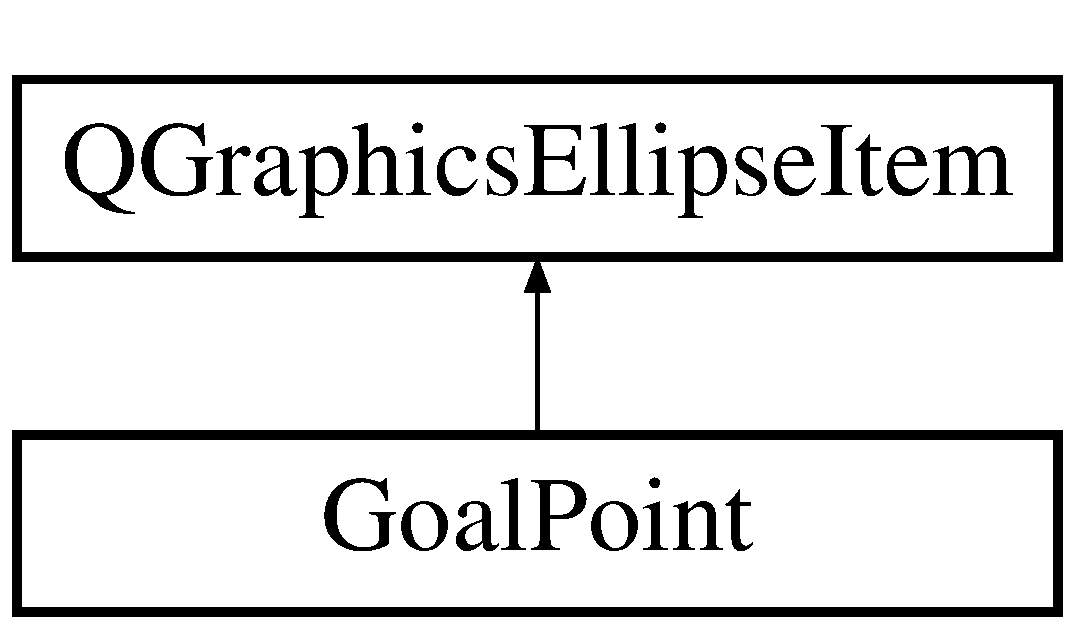
\includegraphics[height=2.000000cm]{class_goal_point}
\end{center}
\end{figure}
\subsection*{Public Member Functions}
\begin{DoxyCompactItemize}
\item 
\hypertarget{class_goal_point_aefa48894f0917222818f8773b2f6459f}{{\bfseries Goal\-Point} (qreal x, qreal y, qreal width, qreal height, Q\-Graphics\-Item $\ast$parent=0)}\label{class_goal_point_aefa48894f0917222818f8773b2f6459f}

\end{DoxyCompactItemize}


The documentation for this class was generated from the following files\-:\begin{DoxyCompactItemize}
\item 
\hyperlink{_goal_point_8h}{Goal\-Point.\-h}\item 
Goal\-Point.\-cpp\end{DoxyCompactItemize}

\hypertarget{class_main_window}{\section{Main\-Window Class Reference}
\label{class_main_window}\index{Main\-Window@{Main\-Window}}
}
Inheritance diagram for Main\-Window\-:\begin{figure}[H]
\begin{center}
\leavevmode
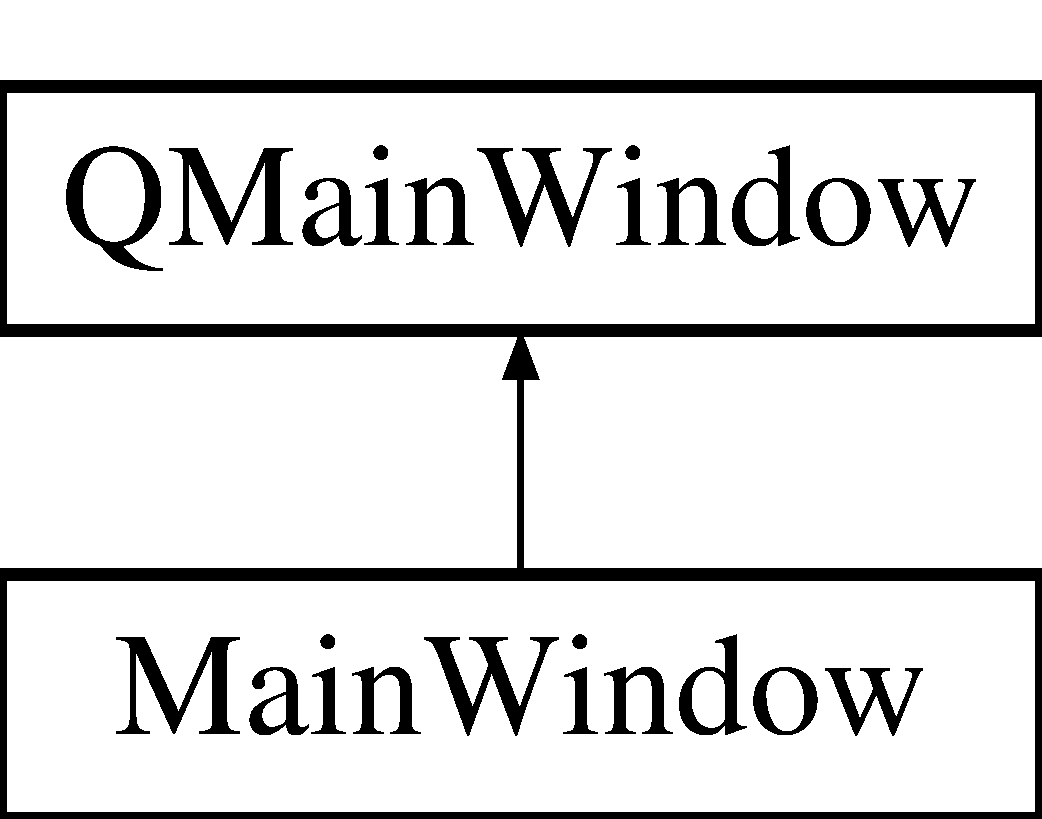
\includegraphics[height=2.000000cm]{class_main_window}
\end{center}
\end{figure}
\subsection*{Public Member Functions}
\begin{DoxyCompactItemize}
\item 
\hypertarget{class_main_window_a232aa83c4ded3b19e4811d00ad9ff842}{{\bfseries Main\-Window} (int agent\-Number, int obstacle\-Number, bool show1\-Field, bool gpu, Q\-Widget $\ast$parent=0)}\label{class_main_window_a232aa83c4ded3b19e4811d00ad9ff842}

\end{DoxyCompactItemize}


The documentation for this class was generated from the following files\-:\begin{DoxyCompactItemize}
\item 
\hyperlink{_main_window_8h}{Main\-Window.\-h}\item 
Main\-Window.\-cpp\end{DoxyCompactItemize}

\hypertarget{class_obstacle}{\section{Obstacle Class Reference}
\label{class_obstacle}\index{Obstacle@{Obstacle}}
}
Inheritance diagram for Obstacle\-:\begin{figure}[H]
\begin{center}
\leavevmode
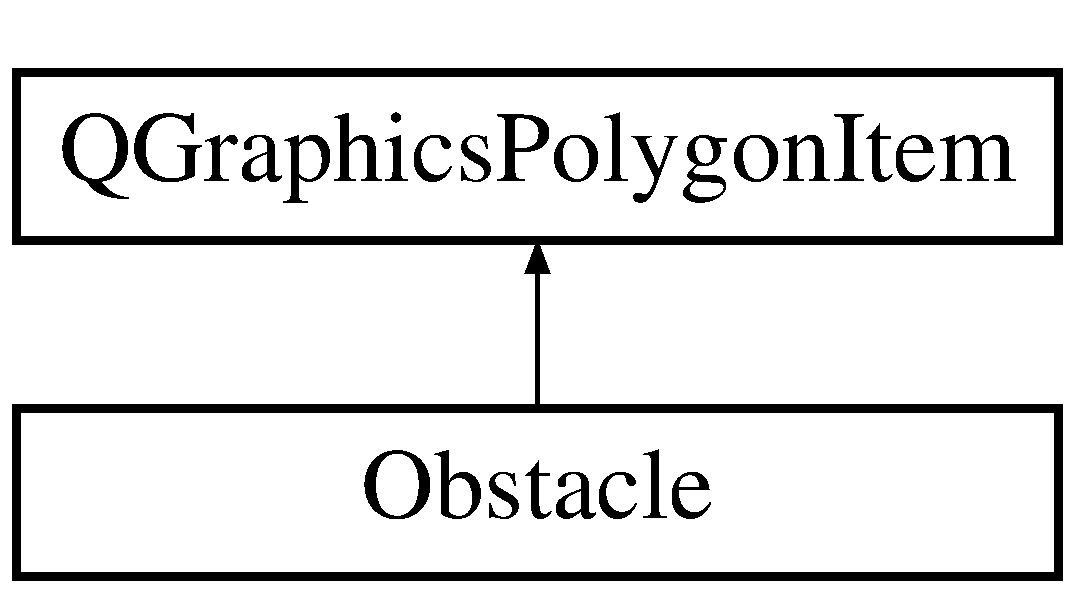
\includegraphics[height=2.000000cm]{class_obstacle}
\end{center}
\end{figure}


The documentation for this class was generated from the following files\-:\begin{DoxyCompactItemize}
\item 
\hyperlink{_obstacle_8h}{Obstacle.\-h}\item 
Obstacle.\-cpp\end{DoxyCompactItemize}

\hypertarget{class_playground}{\section{Playground Class Reference}
\label{class_playground}\index{Playground@{Playground}}
}
Inheritance diagram for Playground\-:\begin{figure}[H]
\begin{center}
\leavevmode
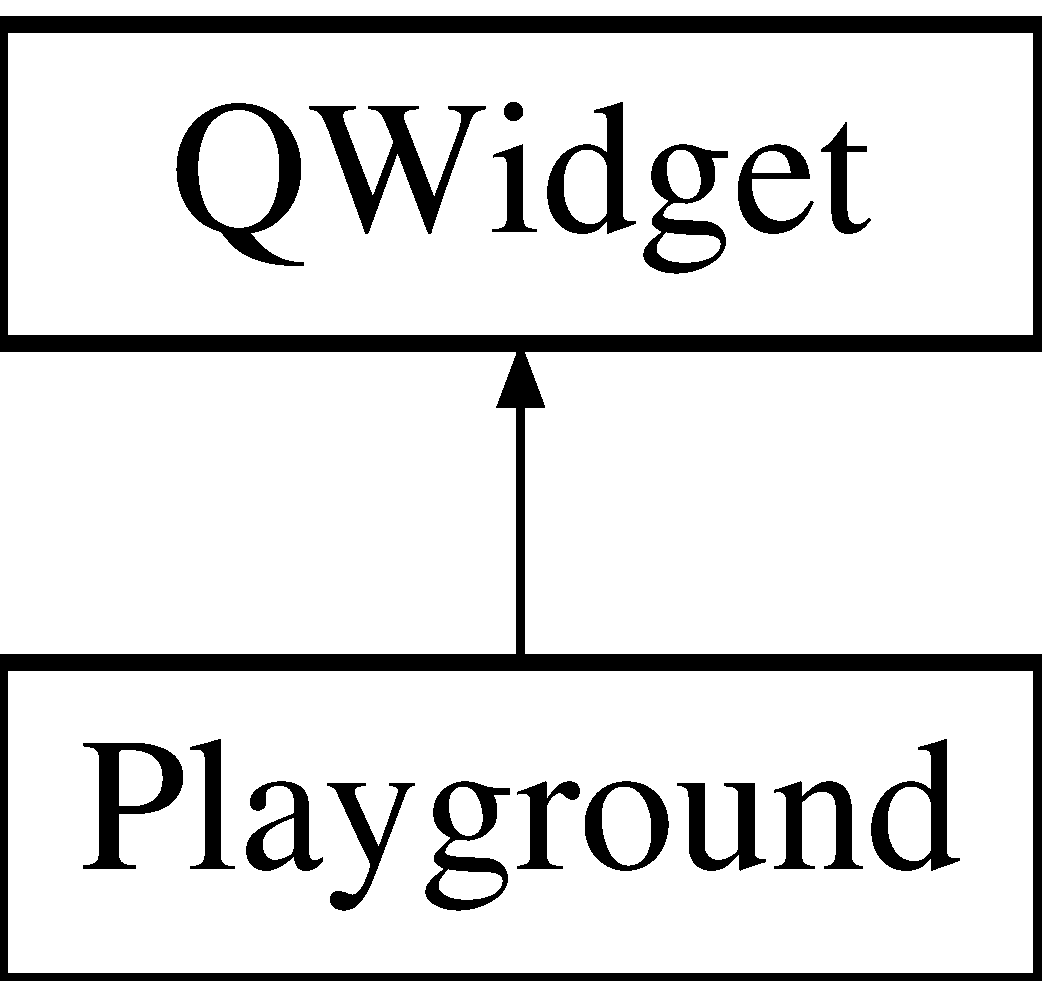
\includegraphics[height=2.000000cm]{class_playground}
\end{center}
\end{figure}
\subsection*{Public Slots}
\begin{DoxyCompactItemize}
\item 
\hypertarget{class_playground_ab3c25c89b13c23be55015f3ab1254714}{void {\bfseries Tick} ()}\label{class_playground_ab3c25c89b13c23be55015f3ab1254714}

\end{DoxyCompactItemize}
\subsection*{Public Member Functions}
\begin{DoxyCompactItemize}
\item 
\hypertarget{class_playground_a69d8c8d62d46a4b35d4c77712d28d534}{{\bfseries Playground} (Q\-Widget $\ast$parent=0, int \-\_\-number\-Agents=10, int \-\_\-number\-Obstacles=50, bool gpu=true)}\label{class_playground_a69d8c8d62d46a4b35d4c77712d28d534}

\item 
\hypertarget{class_playground_ae7a9de301b14f2736ffb7f89796edf6f}{void {\bfseries Set\-Environment} ()}\label{class_playground_ae7a9de301b14f2736ffb7f89796edf6f}

\item 
\hypertarget{class_playground_a9c0b6aeb815da539f130808210e14e17}{void {\bfseries Clear\-Environment} ()}\label{class_playground_a9c0b6aeb815da539f130808210e14e17}

\end{DoxyCompactItemize}


The documentation for this class was generated from the following files\-:\begin{DoxyCompactItemize}
\item 
\hyperlink{_playground_8h}{Playground.\-h}\item 
Playground.\-cpp\end{DoxyCompactItemize}

\hypertarget{struct_point2d}{\section{Point2d Struct Reference}
\label{struct_point2d}\index{Point2d@{Point2d}}
}
\subsection*{Public Attributes}
\begin{DoxyCompactItemize}
\item 
\hypertarget{struct_point2d_a0e2cdd233fb0c476aa03d7faafd8e4bd}{float {\bfseries x}}\label{struct_point2d_a0e2cdd233fb0c476aa03d7faafd8e4bd}

\item 
\hypertarget{struct_point2d_a1ec805cd00047d1e6251167dd55bf2ad}{float {\bfseries y}}\label{struct_point2d_a1ec805cd00047d1e6251167dd55bf2ad}

\end{DoxyCompactItemize}


The documentation for this struct was generated from the following file\-:\begin{DoxyCompactItemize}
\item 
\hyperlink{_triangle_8h}{Triangle.\-h}\end{DoxyCompactItemize}

\hypertarget{class_point2_d}{\section{Point2\-D Class Reference}
\label{class_point2_d}\index{Point2\-D@{Point2\-D}}
}
\subsection*{Public Member Functions}
\begin{DoxyCompactItemize}
\item 
\hypertarget{class_point2_d_a3ad4c92ddc32fbb62c9b189355bd4530}{{\bfseries Point2\-D} (float \-\_\-x, float \-\_\-y)}\label{class_point2_d_a3ad4c92ddc32fbb62c9b189355bd4530}

\item 
\hypertarget{class_point2_d_a6151401987d5f802fa5a03d3936da5ad}{float {\bfseries X} ()}\label{class_point2_d_a6151401987d5f802fa5a03d3936da5ad}

\item 
\hypertarget{class_point2_d_aa736b0dba175039f426f8129a317917b}{float {\bfseries Y} ()}\label{class_point2_d_aa736b0dba175039f426f8129a317917b}

\item 
\hypertarget{class_point2_d_a60b3fea0bd76c3899355fb7048c4e0bc}{void {\bfseries Set} (float \-\_\-x, float \-\_\-y)}\label{class_point2_d_a60b3fea0bd76c3899355fb7048c4e0bc}

\item 
\hypertarget{class_point2_d_a75f1c923356d656782fc21b5590e9744}{float {\bfseries Distance} (const \hyperlink{class_point2_d}{Point2\-D} \&point\-B)}\label{class_point2_d_a75f1c923356d656782fc21b5590e9744}

\item 
\hypertarget{class_point2_d_ac9db38a9b617f6a7871b9501f4ecdc12}{void {\bfseries Set\-Length} (float \-\_\-length)}\label{class_point2_d_ac9db38a9b617f6a7871b9501f4ecdc12}

\end{DoxyCompactItemize}


The documentation for this class was generated from the following files\-:\begin{DoxyCompactItemize}
\item 
\hyperlink{_point2_d_8h}{Point2\-D.\-h}\item 
Point2\-D.\-cpp\end{DoxyCompactItemize}

\hypertarget{class_potential_field}{\section{Potential\-Field Class Reference}
\label{class_potential_field}\index{Potential\-Field@{Potential\-Field}}
}
Inheritance diagram for Potential\-Field\-:\begin{figure}[H]
\begin{center}
\leavevmode
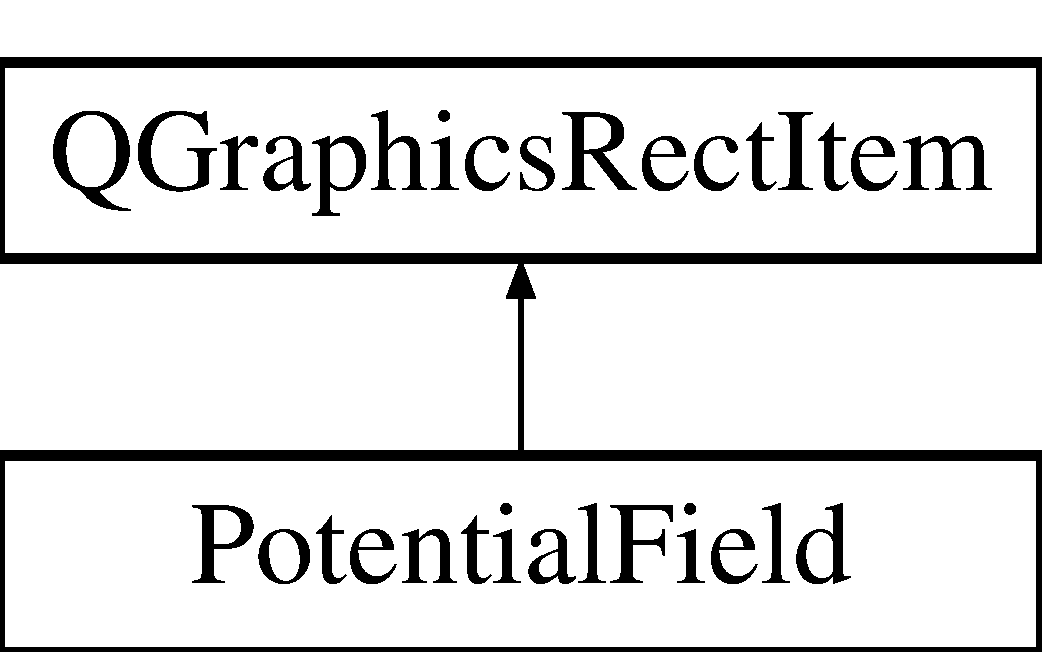
\includegraphics[height=2.000000cm]{class_potential_field}
\end{center}
\end{figure}
\subsection*{Public Member Functions}
\begin{DoxyCompactItemize}
\item 
\hypertarget{class_potential_field_a7b2385c9859061a9fc62f6505f02db52}{{\bfseries Potential\-Field} (\hyperlink{class_agent}{Agent} $\ast$\-\_\-agent, qreal x, qreal y, Q\-Graphics\-Item $\ast$parent=0)}\label{class_potential_field_a7b2385c9859061a9fc62f6505f02db52}

\item 
\hypertarget{class_potential_field_a1fe7dc0a44a503749d1bf800a8daf551}{virtual void {\bfseries paint} (Q\-Painter $\ast$painter, const Q\-Style\-Option\-Graphics\-Item $\ast$option, Q\-Widget $\ast$widget=0)}\label{class_potential_field_a1fe7dc0a44a503749d1bf800a8daf551}

\item 
\hypertarget{class_potential_field_a59152c6e41def1c6623ba28999939cc7}{void {\bfseries Set\-Potential\-Field} (float $\ast$$\ast$\-\_\-potential\-Field, qreal \-\_\-field\-Center\-X, qreal \-\_\-field\-Center\-Y)}\label{class_potential_field_a59152c6e41def1c6623ba28999939cc7}

\end{DoxyCompactItemize}
\subsection*{Static Public Member Functions}
\begin{DoxyCompactItemize}
\item 
\hypertarget{class_potential_field_ab58c950be66b00b911f1cc8cb88f1ceb}{static void {\bfseries Set\-Show1\-Field} (bool show)}\label{class_potential_field_ab58c950be66b00b911f1cc8cb88f1ceb}

\end{DoxyCompactItemize}
\subsection*{Static Public Attributes}
\begin{DoxyCompactItemize}
\item 
\hypertarget{class_potential_field_aed1555fc2d0a42609184f54f8abd16b4}{static const int {\bfseries F\-I\-E\-L\-D\-\_\-\-W\-I\-D\-T\-H} = 64}\label{class_potential_field_aed1555fc2d0a42609184f54f8abd16b4}

\item 
\hypertarget{class_potential_field_a5bc1d7622b1682a58423d75efd0d5074}{static const int {\bfseries T\-I\-L\-E\-\_\-\-W\-I\-D\-T\-H} = 4}\label{class_potential_field_a5bc1d7622b1682a58423d75efd0d5074}

\item 
\hypertarget{class_potential_field_a28d31c5d9ef774ca765e305b16692990}{static const int {\bfseries O\-B\-S\-T\-A\-C\-L\-E} = 100000}\label{class_potential_field_a28d31c5d9ef774ca765e305b16692990}

\end{DoxyCompactItemize}


The documentation for this class was generated from the following files\-:\begin{DoxyCompactItemize}
\item 
\hyperlink{_potential_field_8h}{Potential\-Field.\-h}\item 
Potential\-Field.\-cpp\end{DoxyCompactItemize}

\hypertarget{class_potential_field_worker}{\section{Potential\-Field\-Worker Class Reference}
\label{class_potential_field_worker}\index{Potential\-Field\-Worker@{Potential\-Field\-Worker}}
}
Inheritance diagram for Potential\-Field\-Worker\-:\begin{figure}[H]
\begin{center}
\leavevmode
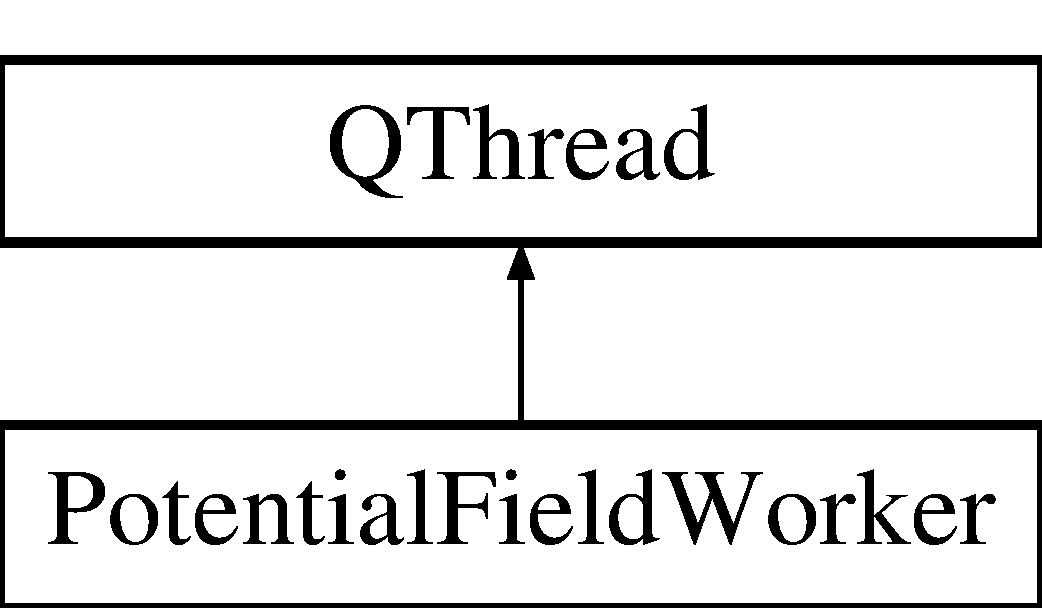
\includegraphics[height=2.000000cm]{class_potential_field_worker}
\end{center}
\end{figure}
\subsection*{Public Member Functions}
\begin{DoxyCompactItemize}
\item 
\hypertarget{class_potential_field_worker_a3c8744a10a2b6eea3f89d2b2e1b175d7}{{\bfseries Potential\-Field\-Worker} (vector$<$ \hyperlink{class_agent}{Agent} $\ast$ $>$ $\ast$\-\_\-agent, vector$<$ \hyperlink{class_obstacle}{Obstacle} $\ast$ $>$ $\ast$\-\_\-obstacle, bool \-\_\-gpu)}\label{class_potential_field_worker_a3c8744a10a2b6eea3f89d2b2e1b175d7}

\item 
\hypertarget{class_potential_field_worker_af199a1a56da40d6d91dac6ace59b91d6}{void {\bfseries Count\-Potential\-Field} (int agent\-I\-D)}\label{class_potential_field_worker_af199a1a56da40d6d91dac6ace59b91d6}

\item 
\hypertarget{class_potential_field_worker_a817c39e54702fcc554cf3d6d53a091ba}{float {\bfseries Count\-Potential\-Field\-Tile} (int agent\-I\-D, int x, int y, int goal\-X, int goal\-Y)}\label{class_potential_field_worker_a817c39e54702fcc554cf3d6d53a091ba}

\item 
\hypertarget{class_potential_field_worker_a15cf6a37f30c755eb9873c23105dd4fb}{float {\bfseries Count\-Potential\-Field\-Tile\-Post\-Process} (int row, int col, float $\ast$$\ast$potential\-Field)}\label{class_potential_field_worker_a15cf6a37f30c755eb9873c23105dd4fb}

\item 
\hypertarget{class_potential_field_worker_a44cedc70fe79f55a8ac8be2af98e2951}{void {\bfseries Send\-Potentional\-Field\-To\-Agent} (int agent\-I\-D, \hyperlink{class_potential_field}{Potential\-Field} $\ast$field)}\label{class_potential_field_worker_a44cedc70fe79f55a8ac8be2af98e2951}

\item 
\hypertarget{class_potential_field_worker_aacbaf877324d41822f30299c4a62b2b0}{void {\bfseries Kill} ()}\label{class_potential_field_worker_aacbaf877324d41822f30299c4a62b2b0}

\item 
\hypertarget{class_potential_field_worker_aacdf2ba9347c1d495bb73201c7cdc67e}{bool {\bfseries Get\-Is\-Finished} ()}\label{class_potential_field_worker_aacdf2ba9347c1d495bb73201c7cdc67e}

\item 
\hypertarget{class_potential_field_worker_ac07ad556aee7ef58d9f00888bbe3613d}{bool {\bfseries Get\-New\-Fields\-Prepared} ()}\label{class_potential_field_worker_ac07ad556aee7ef58d9f00888bbe3613d}

\item 
\hypertarget{class_potential_field_worker_a1ede5ad12775a0f1a402d2cf75190747}{int {\bfseries Get\-Last\-Time\-Elapsed\-M\-S} ()}\label{class_potential_field_worker_a1ede5ad12775a0f1a402d2cf75190747}

\item 
\hypertarget{class_potential_field_worker_a57d837c08330c0745a45c7f5a36c3472}{void {\bfseries Request\-For\-New\-Fields} ()}\label{class_potential_field_worker_a57d837c08330c0745a45c7f5a36c3472}

\item 
\hypertarget{class_potential_field_worker_a9324b452759f542281ed659fadc97229}{void {\bfseries run} ()}\label{class_potential_field_worker_a9324b452759f542281ed659fadc97229}

\end{DoxyCompactItemize}


The documentation for this class was generated from the following files\-:\begin{DoxyCompactItemize}
\item 
\hyperlink{_potential_field_worker_8h}{Potential\-Field\-Worker.\-h}\item 
Potential\-Field\-Worker.\-cpp\end{DoxyCompactItemize}

\hypertarget{struct_triangle}{\section{Triangle Struct Reference}
\label{struct_triangle}\index{Triangle@{Triangle}}
}
\subsection*{Public Attributes}
\begin{DoxyCompactItemize}
\item 
\hypertarget{struct_triangle_a99242d641be48aa814ee08fb2cc8a05d}{\hyperlink{struct_point2d}{Point2d} {\bfseries p} \mbox{[}3\mbox{]}}\label{struct_triangle_a99242d641be48aa814ee08fb2cc8a05d}

\end{DoxyCompactItemize}


The documentation for this struct was generated from the following file\-:\begin{DoxyCompactItemize}
\item 
\hyperlink{_triangle_8h}{Triangle.\-h}\end{DoxyCompactItemize}

\chapter{File Documentation}
\hypertarget{_agent_8h}{\section{Agent.\-h File Reference}
\label{_agent_8h}\index{Agent.\-h@{Agent.\-h}}
}


Contains \hyperlink{class_agent}{Agent} class.  


{\ttfamily \#include $<$Q\-Graphics\-Item$>$}\\*
{\ttfamily \#include $<$queue$>$}\\*
{\ttfamily \#include $<$stack$>$}\\*
{\ttfamily \#include \char`\"{}Point2\-D.\-h\char`\"{}}\\*
\subsection*{Classes}
\begin{DoxyCompactItemize}
\item 
class \hyperlink{class_agent}{Agent}
\begin{DoxyCompactList}\small\item\em Class that holds info about an agent. \end{DoxyCompactList}\end{DoxyCompactItemize}


\subsection{Detailed Description}
Contains \hyperlink{class_agent}{Agent} class. \begin{DoxyAuthor}{Author}
Lukas Beran 
\end{DoxyAuthor}
\begin{DoxyDate}{Date}
2012/11/25 \hyperlink{class_agent}{Agent} class containing necessery methods for moving, painting agent. 
\end{DoxyDate}

\hypertarget{_best_first_search_node_8h}{\section{Best\-First\-Search\-Node.\-h File Reference}
\label{_best_first_search_node_8h}\index{Best\-First\-Search\-Node.\-h@{Best\-First\-Search\-Node.\-h}}
}


Contains \hyperlink{class_best_first_search_node}{Best\-First\-Search\-Node} class.  


\subsection*{Classes}
\begin{DoxyCompactItemize}
\item 
class \hyperlink{class_best_first_search_node}{Best\-First\-Search\-Node}
\end{DoxyCompactItemize}


\subsection{Detailed Description}
Contains \hyperlink{class_best_first_search_node}{Best\-First\-Search\-Node} class. \begin{DoxyAuthor}{Author}
Lukas Beran 
\end{DoxyAuthor}
\begin{DoxyDate}{Date}
2012/11/25 Node class used in A Star path finding. 
\end{DoxyDate}

\hypertarget{_goal_point_8h}{\section{Goal\-Point.\-h File Reference}
\label{_goal_point_8h}\index{Goal\-Point.\-h@{Goal\-Point.\-h}}
}


Contains \hyperlink{class_goal_point}{Goal\-Point} class declaration.  


{\ttfamily \#include $<$Q\-Graphics\-Ellipse\-Item$>$}\\*
\subsection*{Classes}
\begin{DoxyCompactItemize}
\item 
class \hyperlink{class_goal_point}{Goal\-Point}
\end{DoxyCompactItemize}


\subsection{Detailed Description}
Contains \hyperlink{class_goal_point}{Goal\-Point} class declaration. \begin{DoxyAuthor}{Author}
Lukas Beran 
\end{DoxyAuthor}
\begin{DoxyDate}{Date}
2012/11/25 Graphics class to show path ends (goal) of each agent. 
\end{DoxyDate}

\hypertarget{gpu_potential_fields_wrapper_8h}{\section{gpu\-Potential\-Fields\-Wrapper.\-h File Reference}
\label{gpu_potential_fields_wrapper_8h}\index{gpu\-Potential\-Fields\-Wrapper.\-h@{gpu\-Potential\-Fields\-Wrapper.\-h}}
}


Contains functions which uses G\-P\-U.  


\subsection*{Functions}
\begin{DoxyCompactItemize}
\item 
\hypertarget{gpu_potential_fields_wrapper_8h_a3643ad8526895635ea96ac4b5a3eb25e}{void {\bfseries gpu\-Alloc\-Memory} (int \-\_\-number\-Agents, int \-\_\-field\-Width, int \-\_\-tile\-Width)}\label{gpu_potential_fields_wrapper_8h_a3643ad8526895635ea96ac4b5a3eb25e}

\item 
\hypertarget{gpu_potential_fields_wrapper_8h_afc95bcf008abc42530eba4b3a25b96e3}{void {\bfseries gpu\-Alloc\-Obstacles} (int \-\_\-obst\-Area\-Left, int \-\_\-obst\-Area\-Top, int \-\_\-cell\-Width, int \-\_\-cell\-Height, int $\ast$\-\_\-quad\-Tree, \hyperlink{struct_triangle}{Triangle} $\ast$\-\_\-triangle, int triangle\-Size, int $\ast$\-\_\-triangle\-I\-Ds, int triangle\-I\-Ds\-Size)}\label{gpu_potential_fields_wrapper_8h_afc95bcf008abc42530eba4b3a25b96e3}

\item 
\hypertarget{gpu_potential_fields_wrapper_8h_ab08fb7026f717d430230727e6975aec7}{void {\bfseries gpu\-Count\-Potential\-Fields} (float $\ast$$\ast$$\ast$potential\-Field, float $\ast$cpu\-Field\-Center\-X, float $\ast$cpu\-Field\-Center\-Y, int $\ast$cpu\-Goal\-X, int $\ast$cpu\-Goal\-Y)}\label{gpu_potential_fields_wrapper_8h_ab08fb7026f717d430230727e6975aec7}

\item 
\hypertarget{gpu_potential_fields_wrapper_8h_ae4922eb56808f109c5751ca771e84314}{void {\bfseries gpu\-Free\-Memory} ()}\label{gpu_potential_fields_wrapper_8h_ae4922eb56808f109c5751ca771e84314}

\end{DoxyCompactItemize}


\subsection{Detailed Description}
Contains functions which uses G\-P\-U. \begin{DoxyAuthor}{Author}
Lukas Beran 
\end{DoxyAuthor}
\begin{DoxyDate}{Date}
2012/11/25 Methods to allocate, free memory on gpu. For running kernel. 
\end{DoxyDate}

\hypertarget{_main_window_8h}{\section{Main\-Window.\-h File Reference}
\label{_main_window_8h}\index{Main\-Window.\-h@{Main\-Window.\-h}}
}


Contains \hyperlink{class_main_window}{Main\-Window} class.  


{\ttfamily \#include \char`\"{}Playground.\-h\char`\"{}}\\*
{\ttfamily \#include $<$qwidget.\-h$>$}\\*
{\ttfamily \#include $<$Q\-Main\-Window$>$}\\*
\subsection*{Classes}
\begin{DoxyCompactItemize}
\item 
class \hyperlink{class_main_window}{Main\-Window}
\end{DoxyCompactItemize}


\subsection{Detailed Description}
Contains \hyperlink{class_main_window}{Main\-Window} class. \begin{DoxyAuthor}{Author}
Lukas Beran 
\end{DoxyAuthor}
\begin{DoxyDate}{Date}
2012/11/25 Qt main window class. 
\end{DoxyDate}

\hypertarget{_obstacle_8h}{\section{Obstacle.\-h File Reference}
\label{_obstacle_8h}\index{Obstacle.\-h@{Obstacle.\-h}}
}


Contains \hyperlink{class_obstacle}{Obstacle} class.  


{\ttfamily \#include $<$Q\-Graphics\-Item$>$}\\*
\subsection*{Classes}
\begin{DoxyCompactItemize}
\item 
class \hyperlink{class_obstacle}{Obstacle}
\end{DoxyCompactItemize}


\subsection{Detailed Description}
Contains \hyperlink{class_obstacle}{Obstacle} class. \begin{DoxyAuthor}{Author}
Lukas Beran 
\end{DoxyAuthor}
\begin{DoxyDate}{Date}
2012/11/25 \hyperlink{class_obstacle}{Obstacle} graphics item. 
\end{DoxyDate}

\hypertarget{_playground_8h}{\section{Playground.\-h File Reference}
\label{_playground_8h}\index{Playground.\-h@{Playground.\-h}}
}


Contains \hyperlink{class_playground}{Playground} class.  


{\ttfamily \#include $<$Q\-Widget$>$}\\*
{\ttfamily \#include $<$Q\-Timer$>$}\\*
{\ttfamily \#include $<$Q\-Time$>$}\\*
{\ttfamily \#include $<$Q\-Graphics\-Scene.\-h$>$}\\*
{\ttfamily \#include $<$Q\-Graphics\-View.\-h$>$}\\*
{\ttfamily \#include $<$Q\-Graphics\-Item$>$}\\*
{\ttfamily \#include $<$vector$>$}\\*
{\ttfamily \#include $<$Q\-Thread$>$}\\*
{\ttfamily \#include \char`\"{}Potential\-Field\-Worker.\-h\char`\"{}}\\*
{\ttfamily \#include \char`\"{}Agent.\-h\char`\"{}}\\*
{\ttfamily \#include \char`\"{}Obstacle.\-h\char`\"{}}\\*
{\ttfamily \#include \char`\"{}Potential\-Field.\-h\char`\"{}}\\*
{\ttfamily \#include \char`\"{}Goal\-Point.\-h\char`\"{}}\\*
\subsection*{Classes}
\begin{DoxyCompactItemize}
\item 
class \hyperlink{class_playground}{Playground}
\end{DoxyCompactItemize}


\subsection{Detailed Description}
Contains \hyperlink{class_playground}{Playground} class. \begin{DoxyAuthor}{Author}
Lukas Beran 
\end{DoxyAuthor}
\begin{DoxyDate}{Date}
2012/11/25 \hyperlink{class_playground}{Playground} is main class which works with agents, obstacle, potential fields. 
\end{DoxyDate}

\hypertarget{_point2_d_8h}{\section{Point2\-D.\-h File Reference}
\label{_point2_d_8h}\index{Point2\-D.\-h@{Point2\-D.\-h}}
}


Simple \hyperlink{class_point2_d}{Point2\-D} class.  


\subsection*{Classes}
\begin{DoxyCompactItemize}
\item 
class \hyperlink{class_point2_d}{Point2\-D}
\end{DoxyCompactItemize}


\subsection{Detailed Description}
Simple \hyperlink{class_point2_d}{Point2\-D} class. \begin{DoxyAuthor}{Author}
Lukas Beran 
\end{DoxyAuthor}
\begin{DoxyDate}{Date}
2012/11/25 2\-D point containing method Distance to another point and a few usefull methods. 
\end{DoxyDate}

\hypertarget{_potential_field_8h}{\section{Potential\-Field.\-h File Reference}
\label{_potential_field_8h}\index{Potential\-Field.\-h@{Potential\-Field.\-h}}
}


Contains \hyperlink{class_potential_field}{Potential\-Field} class.  


{\ttfamily \#include $<$Q\-Graphics\-Rect\-Item$>$}\\*
{\ttfamily \#include $<$stack$>$}\\*
{\ttfamily \#include $<$Q\-Time$>$}\\*
{\ttfamily \#include \char`\"{}Agent.\-h\char`\"{}}\\*
\subsection*{Classes}
\begin{DoxyCompactItemize}
\item 
class \hyperlink{class_potential_field}{Potential\-Field}
\end{DoxyCompactItemize}


\subsection{Detailed Description}
Contains \hyperlink{class_potential_field}{Potential\-Field} class. \begin{DoxyAuthor}{Author}
Lukas Beran 
\end{DoxyAuthor}
\begin{DoxyDate}{Date}
2012/11/25 Potential field visualisation and method for finding path between agents and the global minimum in the field. 
\end{DoxyDate}

\hypertarget{_potential_field_worker_8h}{\section{Potential\-Field\-Worker.\-h File Reference}
\label{_potential_field_worker_8h}\index{Potential\-Field\-Worker.\-h@{Potential\-Field\-Worker.\-h}}
}


Contains \hyperlink{class_potential_field_worker}{Potential\-Field\-Worker} class for thread.  


{\ttfamily \#include $<$Q\-Thread$>$}\\*
{\ttfamily \#include \char`\"{}Potential\-Field.\-h\char`\"{}}\\*
{\ttfamily \#include \char`\"{}Obstacle.\-h\char`\"{}}\\*
{\ttfamily \#include \char`\"{}Triangle.\-h\char`\"{}}\\*
\subsection*{Classes}
\begin{DoxyCompactItemize}
\item 
class \hyperlink{class_potential_field_worker}{Potential\-Field\-Worker}
\end{DoxyCompactItemize}


\subsection{Detailed Description}
Contains \hyperlink{class_potential_field_worker}{Potential\-Field\-Worker} class for thread. \begin{DoxyAuthor}{Author}
Lukas Beran 
\end{DoxyAuthor}
\begin{DoxyDate}{Date}
2012/11/25 Thread which counts potential fields of agents in the never ending loop 
\end{DoxyDate}

\hypertarget{_triangle_8h}{\section{Triangle.\-h File Reference}
\label{_triangle_8h}\index{Triangle.\-h@{Triangle.\-h}}
}


Contains \hyperlink{struct_triangle}{Triangle} class and few global constants.  


\subsection*{Classes}
\begin{DoxyCompactItemize}
\item 
struct \hyperlink{struct_point2d}{Point2d}
\item 
struct \hyperlink{struct_triangle}{Triangle}
\end{DoxyCompactItemize}
\subsection*{Macros}
\begin{DoxyCompactItemize}
\item 
\hypertarget{_triangle_8h_ae8db1c57b23ae4fe9cdecf63fdb85d47}{\#define {\bfseries A\-R\-E\-A\-\_\-\-C\-E\-L\-L\-\_\-\-W\-I\-D\-T\-H}~8}\label{_triangle_8h_ae8db1c57b23ae4fe9cdecf63fdb85d47}

\item 
\hypertarget{_triangle_8h_aaa523b58073c78b428767f8ba3dd1454}{\#define {\bfseries A\-R\-E\-A\-\_\-\-C\-E\-L\-L\-\_\-\-H\-E\-I\-G\-H\-T}~8}\label{_triangle_8h_aaa523b58073c78b428767f8ba3dd1454}

\item 
\hypertarget{_triangle_8h_a4ca0aad15652b537d986e598208198a8}{\#define {\bfseries M\-A\-X\-\_\-\-T\-R\-I\-A\-N\-G\-L\-E}~1000}\label{_triangle_8h_a4ca0aad15652b537d986e598208198a8}

\item 
\hypertarget{_triangle_8h_a1867378f4c2f78e82e094088efb59425}{\#define {\bfseries M\-A\-X\-\_\-\-T\-R\-I\-A\-N\-G\-L\-E\-\_\-\-I\-D\-S}~4000}\label{_triangle_8h_a1867378f4c2f78e82e094088efb59425}

\end{DoxyCompactItemize}


\subsection{Detailed Description}
Contains \hyperlink{struct_triangle}{Triangle} class and few global constants. \begin{DoxyAuthor}{Author}
Lukas Beran 
\end{DoxyAuthor}
\begin{DoxyDate}{Date}
2012/11/25 Simple triangle struct 
\end{DoxyDate}

\addcontentsline{toc}{part}{Index}
\printindex
\end{document}
